
\documentclass[margin]{res}  

\usepackage{helvet}

\textheight=700pt
\setlength{\textwidth}{5.1in}
\usepackage{graphicx}
\usepackage[export]{adjustbox}
\usepackage{array}
\usepackage{mdframed}


\begin{document}

\name{\Huge Hrishikesh Shedekar \\~}

\address{302 Matoshree Pearl\\Shree Rameshwar CHS\\Opp. Dreams Mall, LBS Marg\\Bhandup(W)\\Mumbai-400078} 

\address{Contact No. +91 9867906725\\
Email id: shedekarhrishi@gmail.com} 


\begin{resume}


\begin{figure}[ht]
    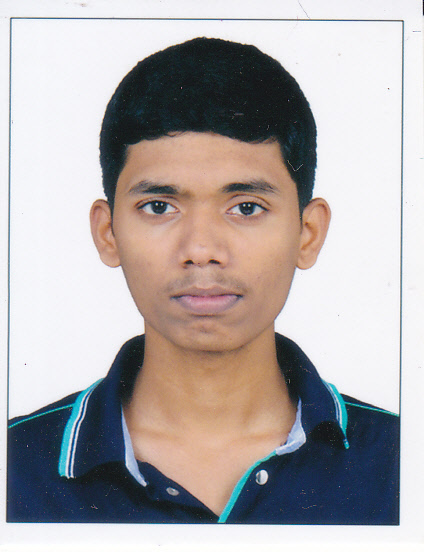
\includegraphics[width=.3\textwidth,right]{me}
\end{figure}

\section{OBJECTIVE}  

To work in a competitive and energetic setting that requires a high level of self-motivation and commitment, allowing me to effectively manage my own professional development and contribute my skills successfully.


\section{EDUCATION}


Pursuing B.E. in Electronics \& Telecommunications Engg. \hfill \(June 2015 - present\)
\begin{flushleft}
\begin{tabular}{ |m{3em}|m{10em}|m{6em}|m{4em}|m{8em}| } 
 \hline
\textbf{Degree} & \textbf{College/ School} & \textbf{University} & \textbf{Passing Year} & \textbf{Pass}\hspace{16mm} \textbf{Percentage}\\
 \hline 
 B.E. & Sardar Patel Institute of Technology & Mumbai \hspace{10mm}University & 2019 & 9.66 CGPA upto Semester 5 \\ 
 \hline
  HSC & Mulund Vidya Mandir Jr, College & Maharashtra State Board & 2015 & 92.15\% \\ 
 \hline
 SSC & St. Xavier's High School & Maharashtra State Board & 2013 & 94.36\% \\ 
 \hline
 
\end{tabular}
\end{flushleft}

\section{PROJECTS} 


\begin{enumerate}
   \item \textbf{Vehiclular Accident prevention system} \hfill \(Feb,18 - April,18\)\\
   \textbf{based on Cognitive driving Distraction}\\
   Worked as the Technical Head, to develop a system that works towards prevention of accidents caused mainly due to human errors by monitoring the driver's behavioural and physiological features like Drowsiness, Stress, Anxiety and influence of Alcohol and then takes preventive actions.\\

\item \textbf{Collector Bot: e-Yantra Robotics Compeition} \hfill \(Oct,17 - March,18\)\\
   Worked on Image Processing using Python OpenCV, Path Planning and motion planning in V-Rep, implementing PID algorithm and Robot Structure design. \\The theme of this project is to detect and collect fruits in shortest possible time, using efficient paths to avoid collisions with obstacles. \\

   \item \textbf{High-Resolution Microstepping Controller }                           \hfill \(Dec,2017-Jan,2018\)\\
This project involves designing a High-resolution Microstepping Controller to implement Microstepping which is a way of moving the stator flux of a stepper more smoothly than in full- or half-step drive modes, used to achieve higher resolution or smoother motion at low speeds.  \\

   \item \textbf{4G Technology Based Data Acquisition System}                     \hfill             \(Aug,2017-Nov,2017\)\\
The system involves a SIM7100 4G module interfaced to an Atmega8535 Microcontroller, where the current output of a remote system is measured using a Hall effect based sensor and this data is logged \& stored in an SD card, and the efficiency of the Machines is calculated and relevant SMS alerts are sent using 4G technology. 


\item \textbf{ e-Nirogya : an IoT based Health Care System}                     \hfill             \(Jan,2017-July,2017\)\\
e-Nirogya is a remote health monitoring system for Rural Areas which uses a Raspberry Pi as the Central processor to collect Critical Health parameter data for remote diagnosis of diseases and immediate medical consultation from Urban Doctors.\\
Worked as the Technical Head,developed and implemented the Hardware System and mechanism for uploading data from remote locations and performing Online Data Analytics.   

\end{enumerate}

\section{TRAINING \&\\ INTERNSHIPS}
\begin{itemize}
  \item Winter \textbf{Internship} at TATA INSTITUE OF FUNDAMENTAL RESEARCH \textbf{$($TIFR$)$ }\hfill \textit{Duration: 1 Month $($Dec,17 - Jan,18$)$} \\
 Worked as an intern at ECR lab,Department of Nuclear and Atomic Physics, TIFR
  
  \item \textbf{Embedded Systems Design Training Course} \hfill \textit{Duration: 3 Months $($Nov,16 - Jan,17$)$} \\
 Worked on AVR, ARM, MSP based micro controllers systems and interfacing these with wireless communication modules, ESP-8266, SIM908
  
\end{itemize}

\section{TECHNICAL SKILLS}
\begin{enumerate}

\item \textbf{Programming Languages} : C $|$ Embedded C $|$  Python $|$  JAVA $($Basics$)$ 
\item \textbf{Softwares}: AVR Studio $|$ V-Rep $|$ XCTU $|$ MATLAB $|$ Keil $|$ Eagle PCB Design $|$ Linux $|$ AutoCAD $|$ Cisco Packet Tracer $|$ Scilab $|$ PSPICE


\end{enumerate}

\section{SOFT SKILLS}
\begin{itemize}

\item Good Communication Skills
\item Leadership \& Teamwork
\item Time Management
\item Creativity \& Adaptibility

\end{itemize}

\end{resume}
\end{document}